\documentclass{beamer}
\setbeamersize{text margin left=3mm,text margin right=3mm}

\mode<presentation> {
	% \usetheme{Montpellier}
	\usetheme{Singapore}
	\usepackage{subcaption}
	\usecolortheme{seahorse}
}

\usepackage{graphicx}
\setbeamertemplate{footline}[frame number]

\usepackage[polish]{babel}
\usepackage[utf8x]{inputenc}
\usepackage{caption}
\usepackage{hyperref}
\usepackage{polski}
\usepackage{polski}

\title[analiza stężenia PM2.5]{Analiza stężenia pyłu PM2.5 w Pekinie, \\ lata 2010-2014}

\author{Jakub Pokrywka}
\institute[]
{\medskip
	\textit{jakubpokrywka@gmail.com} % Your email address
}
\date{\today}

\begin{document}

\begin{frame}
	\titlepage
\end{frame}

\section{analiza szeregu czasowego}
\begin{frame}
	Dane przedstawiają cogodzinny zapis stężenia cząsteczki PM2.5 oraz danych atmosferycznych w Pekinie, w latach 2010-2014.
	Po analizie zbioru jako szeregu czasowego nasuwają się następujące wnioski:
	\begin{itemize}
		\item Brak wyraźnej okresowości wysokości stężenia w zależności od godziny,
		\item średnia okresowość wysokości stężenia w zależności od miesiąca. Najwyższe stężenia zaobserwować można w okresie październik-luty.
			Prawdopodobnie jest to wynikiem sezonu grzewczego.
			Podejrzanie niska wartość na wykresie dla stycznia 2011 wynika z braku danych w tym miesiącu (90\% braków).
		\item nie ma trendu zmiany średniego stężenia na przestrzeni lat.
	\end{itemize}
\end{frame}

\begin{frame}
	\begin{figure}
		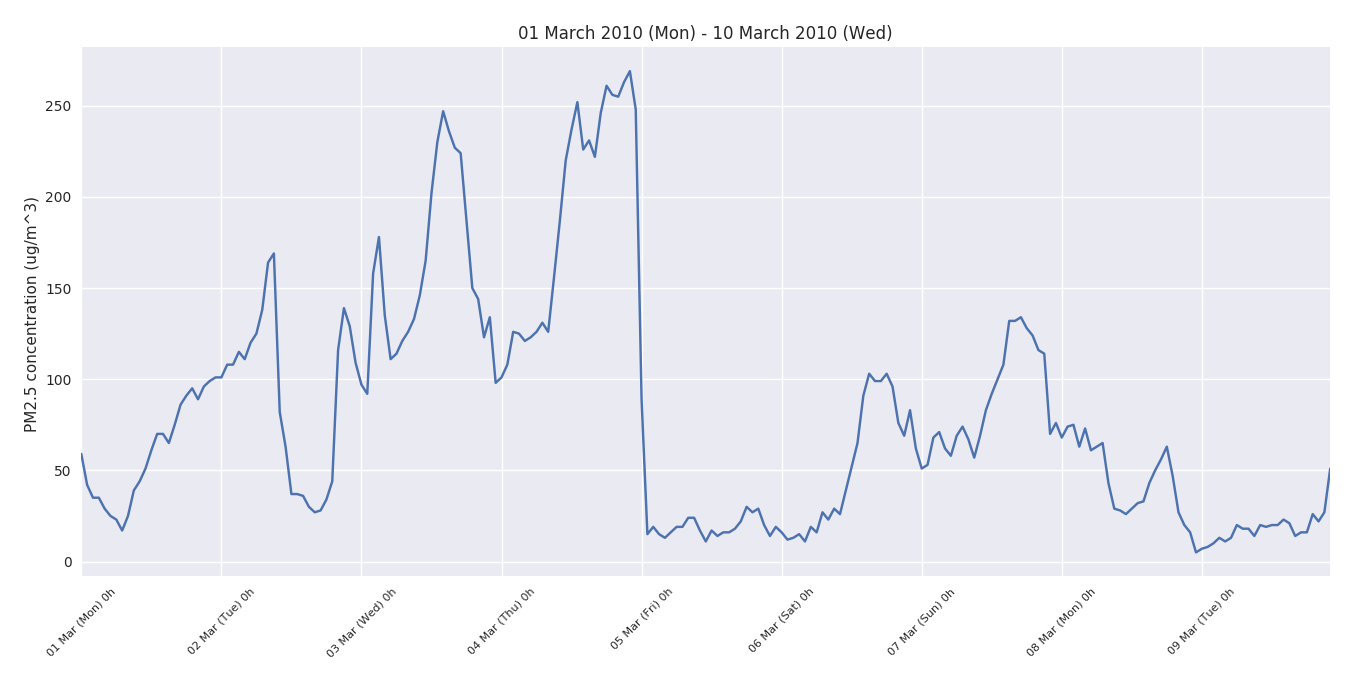
\includegraphics[width=1\linewidth]{time-period}
	\end{figure}
\end{frame}


\begin{frame}
	\begin{figure}
		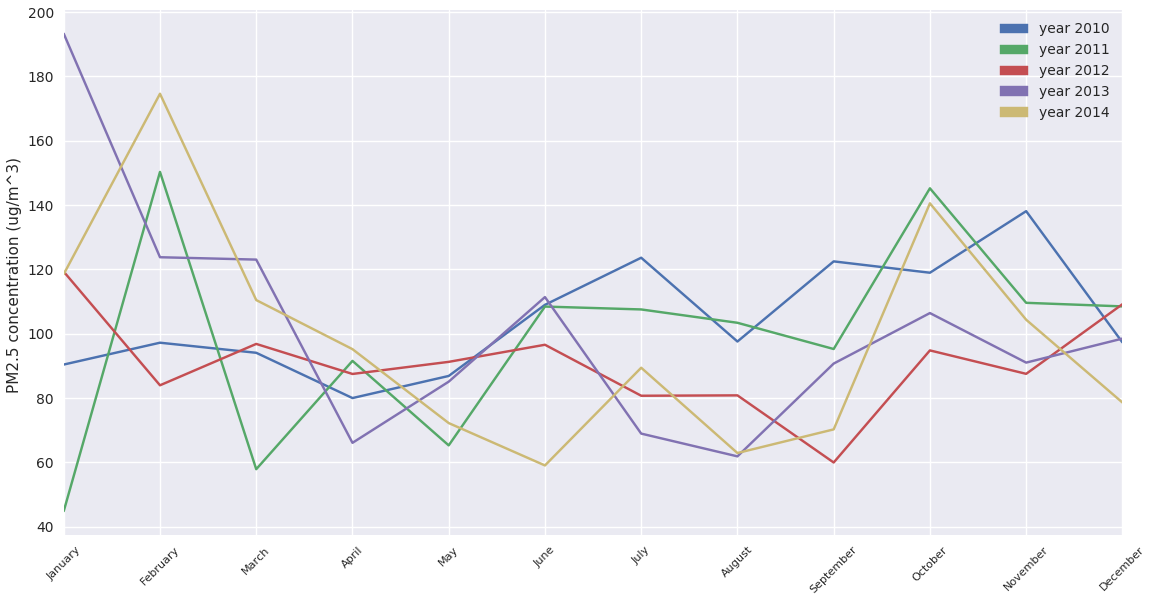
\includegraphics[width=1\linewidth]{month-years}
	\end{figure}
\end{frame}


\section{wpływ warunków atmosferycznych}
\begin{frame}
	Widoczny jest natomiast duży wpływ warunków atmfosferycznych na wartość stężenia PM2.5. Występuje korelacja dodatnia między PM2.5, a punktem rosy (DEWP- wsp. korelacji 0.17),
	co wiąże się ze zmianą wilgotności. Wpływ prędkości wiatru (Iws) jest istotny- nim większy, tym mniejsze stężenie. (wsp. korelacji -0.25). Kierunek wiatru ma pozorny wpływ na wartość stężenia (wynika to z nierównomiernego natężenia wiatru z różnych stron).
	\begin{figure}
		\centering
		\begin{minipage}{.5\textwidth}
			\centering
			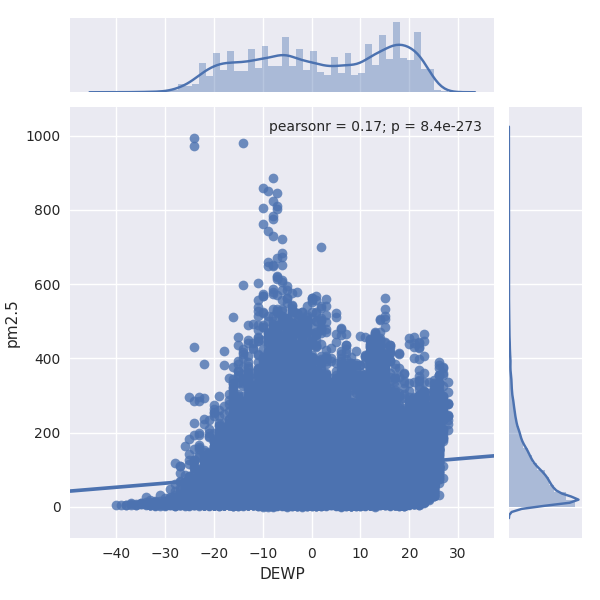
\includegraphics[width=0.7\linewidth]{dewp}
		\end{minipage}%
		\begin{minipage}{.5\textwidth}
			\centering
			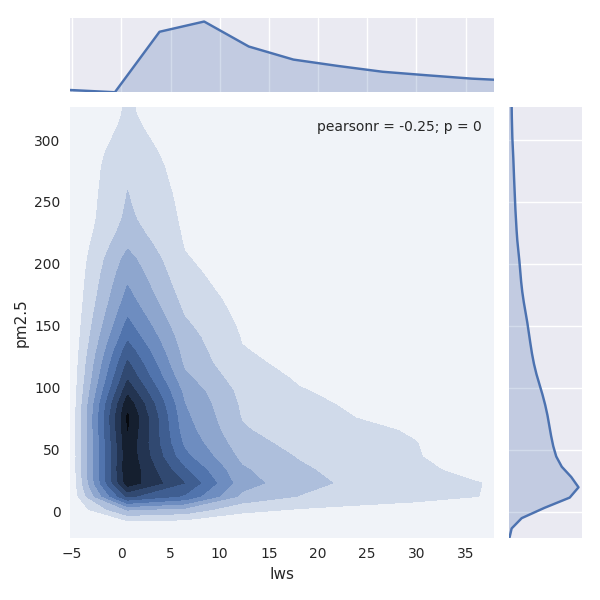
\includegraphics[width=0.7\linewidth]{Iws}
		\end{minipage}
	\end{figure}

\end{frame}



\section{model predykcyjny}
\begin{frame}
	W celu przewidzenia stężenia PM2.5 stworzono model regresji liniowej oraz model neuronowy. Dla obu modeli najlepszy okazał się zestaw cech:
	miesiąc, godzina, punkt rosy, temperatura, ciśnienie, prędkość wiatru, czas opadu śniegu, czasu opadu deszczu, kierunek wiatru (zakodowawany jako wektor binarny).
	\begin{itemize}
		\item Naiwny model (zawsze średnia) daje MSE równe 8257
		\item Model regresji liniowej daje MSE równe 6051
		\item Model neuronowy (5 warstw ukrytych) daje MSE 4791 z odchyleniem standardowym 267 (walidacja krzyżowa z podziałem 0.1)
	\end{itemize}
	Ze względu na wielkość zbioru, model neuronowy daje zdecydowanie lepszy wynik niż prosta regresja liniowa,
	zatem w tym przypadku jest rekomendowany.
\end{frame}

\end{document}
